\documentclass[12pt]{beamer}
\newenvironment{ConCodigo}[1]
  {\begin{frame}[fragile,environment=ConCodigo]{#1}}
  {\end{frame}}
\graphicspath{{Imagenes/}{../Imagenes/}}
\usepackage[utf8]{inputenc}
\usepackage[spanish]{babel}
\usepackage{hyperref}
\usepackage{etex}
%\reserveinserts{28}
\usepackage{amsmath}
\usepackage{amsthm}
\usepackage{mathtools}
\usepackage{multicol}
\usepackage{multirow}
\usepackage{tabulary}
\usepackage{booktabs}
\usepackage{nccmath}
\usepackage{physics}
\usepackage{biblatex}
\usepackage[outdir=./]{epstopdf}
%\epstopdfsetup{outdir=./}
\usepackage{graphicx}
%\usepackage{enumitem,xcolor}
\usepackage{siunitx}
%\sisetup{scientific-notation=true}
%\usepackage{fontspec}
\usepackage{lmodern}
\usepackage{float}
\usepackage[format=hang, font=footnotesize, labelformat=parens]{caption}
\usepackage[autostyle,spanish=mexican]{csquotes}
\usepackage{standalone}
\usepackage{blkarray}
\usepackage{algorithm}
\usepackage{algorithmic}
\usepackage{tikz}
\usepackage[siunitx, RPvoltages]{circuitikz}
\usetikzlibrary{arrows,patterns,shapes}
\usetikzlibrary{decorations.markings}
\usetikzlibrary{arrows}
\usepackage{color}
\usepackage{xcolor}
%\usepackage{beton}
%\usepackage{euler}
%\usepackage[T1]{fontenc}
\usepackage[sfdefault]{roboto}  %% Option 'sfdefault' only if the base font of the document is to be sans serif
\usepackage[T1]{fontenc}
\renewcommand*\familydefault{\sfdefault}
\DeclareGraphicsExtensions{.pdf,.png,.jpg}
\usepackage{hyperref}
\renewcommand {\arraystretch}{1.5}
\newcommand{\python}{\texttt{python}}
\usefonttheme[onlymath]{serif}
\setbeamertemplate{navigation symbols}{}
\usetikzlibrary{patterns}
\usetikzlibrary{decorations.markings}
\tikzstyle{every picture}+=[remember picture,baseline]
%\tikzstyle{every node}+=[inner sep=0pt,anchor=base,
%minimum width=2.2cm,align=center,text depth=.15ex,outer sep=1.5pt]
%\tikzstyle{every path}+=[thick, rounded corners]
\setbeamertemplate{caption}[numbered]
\newcommand{\ptm}{\fontfamily{ptm}\selectfont}
%Se usa la plantilla Warsaw modificada con spruce
\mode<presentation>
{
  \usetheme{Warsaw}
  \setbeamertemplate{headline}{}
  \useoutertheme{default}
  \usecolortheme{albatross}
  \setbeamercovered{invisible}
}
% \AtBeginSection[]
% {
% \begin{frame}<beamer>{Contenido}
% \normalfont\mdseries
% \tableofcontents[currentsection]
% \end{frame}
% }

\include{pre_codigo}
\title{Tema 2 - Operaciones matemáticas básicas}
\subtitle{Cálculo de raíces II}
\author[]{M. en C. Gustavo Contreras Mayén}
\begin{document}
\maketitle
\fontsize{14}{14}\selectfont
\spanishdecimal{.}
\begin{frame}{Contenido}
\tableofcontents[pausesections]
\end{frame}
\section{Método de Newton-Raphson}
\begin{frame}
\frametitle{Método de Newton-Raphson}
El método de Newton-Raphson es el algoritmo más conocido para encontrar raíces por una buena razón: es simple y rápido.
\\
\medskip
El único detalle es que utiliza la derivada $f'(x)$ así como la función $f(x)$. Por tanto, en los problemas a resolver con este algoritmo, deberá de contemplarse que la derivada sea fácil de calcularse.
\end{frame}
\begin{frame}
El método de N-R se obtiene de la expansión en series de Taylor de $f(x)$ alrededor de $x$:
\[ f(x_{i+1})  = f(x_{i})+ f'(x_{i})(x_{i+1}-x_{i}) + O(x_{i+1}-x_{i})^{2}\]
\end{frame}
\begin{frame}
Si $x_{i+1}$ es una raíz de $f(x)=0$, tenemos que:
\[ 0 = f(x_{i}) + f'(x_{i})(x_{i+1}-x_{i})+ O(x_{i+1}-x_{i})^{2} \]
Suponiendo que $x_{i}$ está cerca de $x_{i+1}$, podemos eliminar el último término de la ecuación y resolver para $x_{i+1}$, por lo que la fórmula de Newton-Raphson es:
\[ x_{i+1} = x_{i} - \dfrac{f(x_{i})}{f'(x_{i})} \]
\end{frame}
\begin{frame}
Si $x$ representa el valor verdadero de la raíz, el error en $x_{i}$ es $E_{i}=x-x_{i}$. Se puede demostrar que si $x_{i+1}$ se calcula de la expresión de N-R, el error es:
\[ E_{i+1} = - \dfrac{f''(x_{i})}{2 f'(x_{i})} E_{i}^{2}\]
Lo que nos dice que el método de N-R converge de manera cuadrática, es decir, el error es el cuadrado del error del punto previo.
\end{frame}
\begin{frame}[fragile]
\frametitle{Representación gráfica}
Podemos interpretar que $x_{i+1}$ es el punto en donde la tangente de $f(x_{i})$ cruza el eje de las $x$:
\begin{center}
	\begin{tikzpicture}[font=\small, scale=0.8]
		\draw [->] (0,0) -- (7,0);
		\draw [<->] (0,-3) -- (0,3);
		\draw [red] (1,3) .. controls (1.5,0.5) and (5,-2) .. (6.5,-2);
		\draw (1,-0.3) node {$x_{i}$};
		\draw (1,3.3) node {$f(x_{i})$};
		\draw [dashed] (1.2,0) -- (1.2,2.35);
		\draw (0.8,3.1) -- (2.35,-0.1);
		\draw [dashed] (2.3,0) -- (2.3,0.58);
		\draw (2.3,-0.3) node {$x_{i+1}$};
	\end{tikzpicture}
\end{center}
\end{frame}
\begin{frame}
El método de N-R es sencillo: se aplica la expresión para $x_{i+1}$ iniciando con un valor $x_{0}$, hasta alcanzar un criterio de convergencia:
\[ \vert x_{i+1} - x_{i} \vert < \epsilon \]
El algoritmo es el siguiente:
\begin{enumerate}
\item Sea $x$ un valor inicial para la raíz de $f(x)=0$.
\item Calcular $\Delta x = - f(x)/f'(x)$.
\item Asignar $x \leftarrow x + \Delta x$ y se repiten los pasos 2-3, hasta alcanzar $\vert \Delta x \vert < \epsilon$.
\end{enumerate}
\end{frame}
\begin{frame}[fragile]
Aunque el método de Newton-Raphson converge rápidamente cerca de la raíz, sus características globales de convergencia son pobres. La razón es que la línea tangente no es siempre una aproximación aceptable de la función.
\end{frame}
\begin{frame}[fragile]
\begin{center}
	\begin{tikzpicture}[font=\small, scale=0.8]
		\draw [->] (0,0) -- (4,0);
		\draw [<->] (0,-1) -- (0,3);
		\draw [red] (1,3) .. controls (2,3) and (2.5,2) .. (3.5,-2);
		\draw (1.2,3) circle (0.05);
		\draw [blue, ->] (1.2,3) -- (3.5,2.7);
		\draw (4.2,0) node {$x$};
		\draw (-0.5,2) node {$f(x)$};
		\draw [dashed] (1.2,0) -- (1.2,3);
		\draw (1.2,-0.2) node {$x_{0}$};
	\end{tikzpicture}
\end{center}
\end{frame}
\begin{frame}[fragile]
\begin{center}
\setbeamercovered{invisible}
	\begin{tikzpicture}[decoration={
  markings,% activar las marcas
  mark= at position 2cm with{\arrow{stealth}}}]
		\draw [->] (0,0) -- (6,0);
		\draw [<->] (0,-2) -- (0,2);
		\draw [red] (0.5,-2) .. controls (3,-1.9) and (3,1.9) .. (5.5,2);
		\draw (4.5,-0.3) node {$x_{0}$};\pause
		\draw [dashed] (4.5,0) -- (4.5,1.69);
		\draw (4.5,1.7) circle (0.04);
		\draw [blue, postaction={decorate}] (4.5,1.7) -- (1,0);
		\draw (1,0.3) node {$x_{1}$};
		\draw (1,0) circle (0.04);\pause
		\draw [dashed] (1,0) -- (1,-1.95);
		\draw (1,-1.95) circle (0.04);
		\draw [blue,, postaction={decorate}] (1,-1.95) -- (5.8,0.1);
	\end{tikzpicture}
\end{center}
\end{frame}
\subsection{Algoritmo para el método Newton-Raphson}
\begin{frame}
\frametitle{Algoritmo para el método Newton-Raphson}
La siguiente algoritmo para el método de Newton-Raphson supone que la raíz a calcularse inicialmente está en el intervalo (a, b).
\\
\medskip
El punto medio del intervalo se utiliza como aproximación inicial de la raíz. Los extremos del intervalo se actualizan luego de cada iteración. Si una iteración del método Newton-Raphson no se mantiene dentro del intervalo, se descarta y se reemplaza
con el método de bisección.
\\
\medskip
Ya que el método \texttt{newtonRaphson} utiliza la función $f(x)$, así como su derivada, (denotadas por $f$ y $df$) deben ser proporcionadas por
el usuario.
\end{frame}
\begin{frame}[fragile]
\frametitle{Algoritmo de \texttt{Newton-Raphson}, versión larga}
\begin{lstlisting}
def newtonRaphson(f,df,a,b,tol=1.0e-9):
    fa = (f(a)
    if fa == 0.0: return a
    fb = f(b)
    if f(b) == 0.0: return b
    if fa*fb > 0.0: print 'La raiz no esta en el intervalo'
    x = 0.5 * (a + b)
\end{lstlisting}
\end{frame}
\begin{frame}[fragile]
\begin{lstlisting}
    for i in range(30):
        fx = f(x)
        if abs(fx) < tol: return x

        if fa*fx < 0.0:
            b = x
        else:
            a = x; fa = fx
\end{lstlisting}
\end{frame}
\begin{frame}[fragile]
\begin{lstlisting}
        dfx = df(x)
        
        try: dx = -fx/dfx
        except ZeroDivisionError: dx = b - a
        x =  x + dx
        
        if(b - x)*(x - a) < 0.0:
            dx = 0.5*(b-a)
            x = a + dx
        
        if abs(dx) < tol*max(abs(b),1.0): return x
    
    print 'Son demasiadas iteraciones'
\end{lstlisting}
\end{frame}
\begin{frame}
\frametitle{Ejercicio}
Encontrar la raíz positiva más pequeña de
\[ f(x) = x^{4} - 6.4 x^{3} + 6.45x^{2} + 20.538x - 31.752\]
\begin{figure}
	\centering
	\visible<2-> {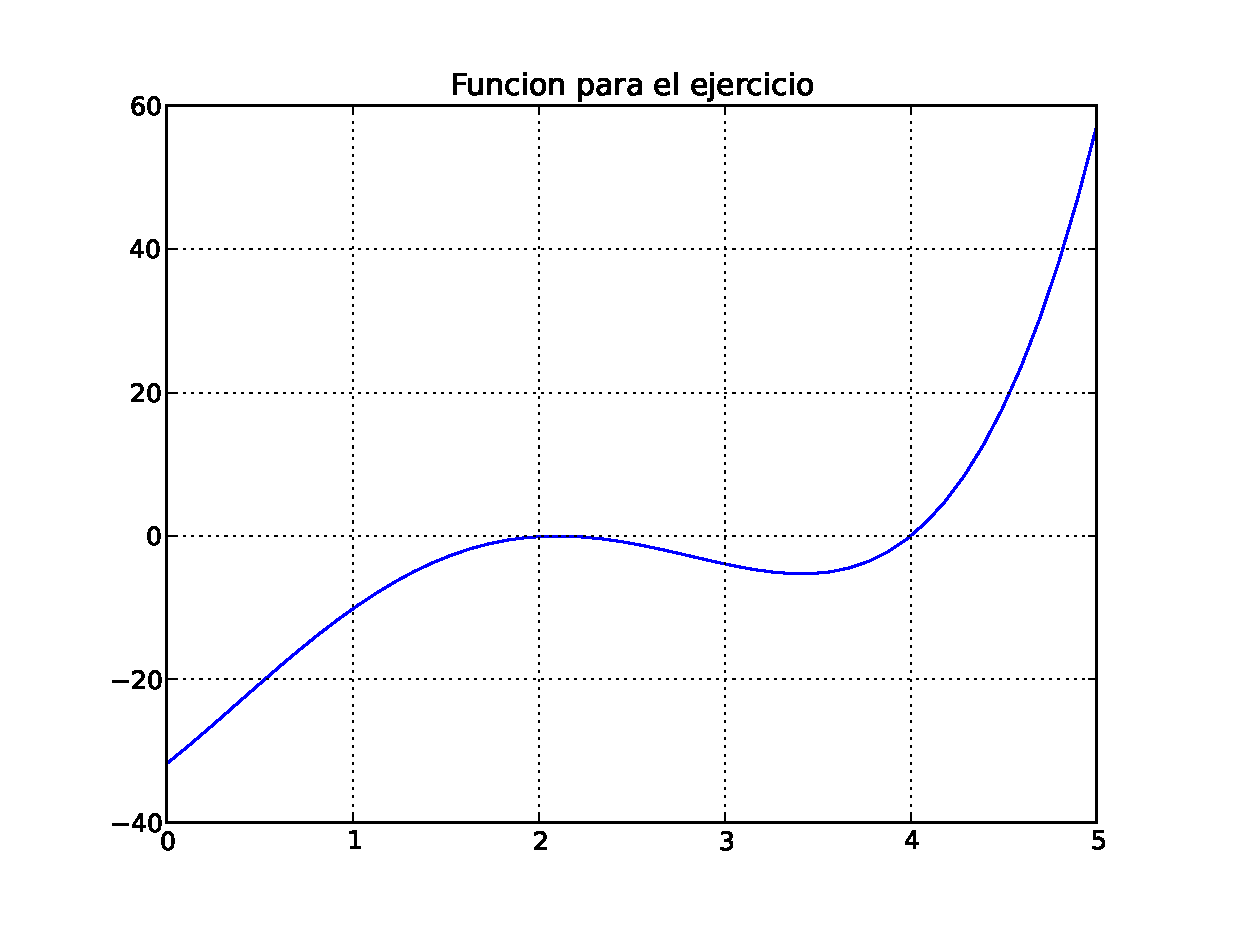
\includegraphics[scale=0.3]{raices08.eps}}
\end{figure}
\end{frame}
\begin{frame}[fragile]
\frametitle{Versión corta del algoritmo}
Revisa que esta versión del algoritmo, sólo requiere de dos argumentos: $x$ la aproximación inicial y $tol$ la tolerancia de corte.
\begin{lstlisting}
def f(x): return x**4 - 6.4*x**3 + 6.45*x**2 + 20.538*x - 31.752
def df(x): return 4.0*x**3 - 19.2*x**2 + 12.9*x + 20.538

def newtonRaphson(x,tol=1e-05):
    for i in range(30):
        dx = -f(x)/df(x)
        x = x + dx
        if abs(dx) < tol: return x,i
    print 'Son demasiadas iteraciones\n'

raiz,numIter = newtonRaphson(2.0)

print 'Raiz =',raiz
print 'Numero de iteraciones =',numIter
\end{lstlisting}
\end{frame}
\begin{frame}
\frametitle{Ejercicios a cuenta.}
\begin{enumerate}
\item Encuentra las raíces de $x \sin x + 3 \cos x - x = 0$ en el intervalo $(-6,6)$ \\
\item Calcula todas las raíces reales de $x^{4} + 0.9x^{3} - 2.3x^{2} + 3.6x - 25.2 = 0$. \\
\item Calcula todas las raíces reales de $x^{4} + 2x^{3} - 7x^{2} + 3 = 0$. \\
\item Calcula todas las raíces de $\sin x - 0.1x = 0$.
\end{enumerate}
\end{frame}
\begin{frame}
\frametitle{Metodología a seguir}
Para la solución de cada uno de los ejercicios, un proceso de solución podría ser el siguiente:
\begin{enumerate}
\item Graficar la función para conocer el comportamiento. Si conocemos el intervalo de solución, podremos acotar la gráfica, pero en caso contrario, debemos explorar para revisar y considerar un intervalo de operación más adecuado.
\item Conocer los intervalos donde hay una raíz. El método de incrementos sucesivos nos permite conocer un intervalo donde se encuentra una raíz, debemos de ajustar el código para que nos devuelva el(los) intervalo(s) donde hay una raíz, para ocupar éstos intervalos posteriomente en el algoritmo de Newton-Raphson.
\end{enumerate}
\end{frame}
\begin{frame}
\begin{enumerate}
\frametitle{Metodología a seguir}
\item Iterar el algoritmo en cada intervalo donde hay una raíz. Como ya conocemos los intervalos con raíz, nuestro siguiente paso es usar el algoritmo para que de manera automática, nos devuelva el valor de la raíz, básicamente hay que recorrer el objeto en donde almacenamos los pares de puntos del intervalo con raíz.
\item Graficar la raíz. Como ya conocemos el valor de la raíz, podemos agregarlo a la gráfica de la función y obtener de manera autómatica la representación de la raíz.
\end{enumerate}
\end{frame}
\section{Método de la falsa posición}
\begin{frame}
\frametitle{Método de la falsa posición}
Este método es parecido al de bisección, ya que el intervalo que contiene a la raíz se va reduciendo.
\\
\bigskip
En vez de bisectar de manera monótona el intervalo, se utiliza una interpolación lineal ajustada a dos puntos extremos para encontrar la aproximación de la raíz.
\end{frame}
\begin{frame}[fragile]
\frametitle{Método de la falsa posición}
\begin{center}
	\begin{tikzpicture}[font=\small]
		\draw [->] (0,0) -- (7,0);
		\draw [<->](0,-3) -- (0,3);
		\draw [red] (1,3) .. controls (1.5,0.5) and (5,-2) .. (6.5,-2);
		\draw (1.2,-0.3) node {$a$};
		\draw (6.3,0.3) node {$c$};
		\draw [dashed] (1.2,0) -- (1.2,2.35);
		\draw [dashed] (6.3,0) -- (6.3,-1.98);
		\draw (0.6,2.2) node {$f(a)$};
		\draw (6.8,-1.9) node {$f(c)$};
		\draw (1.2,2.35) -- (6.3,-1.98);
		\draw  (3,3) node {Interpolación lineal};
		%\draw [->] (3,2.6) -- (2,2);
		%\draw  (5,1) node {1a. aproximación};
		%\draw [->] (5,0.6) -- (4.1,0.1);
		%\draw [dashed] (4,0) -- (4,-0.9);
	\end{tikzpicture}
\end{center}
\end{frame}
\begin{frame}
La función está bien aproximada por la interpolación lineal, con lo que las raíces tendrán una buena precisión; la iteración convergerá más rápido que como ocurre con el método de bisección.
\end{frame}
\begin{frame}
Dado un intervalo $[a,c]$ que contenga a la raíz, la función lineal que pasa por $(a,f(a))$ y $(c,f(c))$ se escribe como:
\[ y = f(a) + \dfrac{f(c)-f(a)}{c-a}(x-a) \]
de donde se despeja $x$:
\[ x = a + \dfrac{c-a}{f(c)-f(a)}(y-f(a)) \]
\end{frame}
\begin{frame}
La coordenada $x$ en donde la línea intersecta al eje $x$ se determina al hacer $y=0$ en la ecuación anterior, por tanto:
\[ b = a - \dfrac{c-a}{f(c)-f(a)}f(a) = \dfrac{af(c)-cf(a)}{f(c)-f(a)} \]
\end{frame}
\begin{frame}[fragile]
\frametitle{Método de la falsa posición}
\begin{center}
	\begin{tikzpicture}[font=\small]
		\draw [->] (0,0) -- (7,0);
		\draw [<->](0,-3) -- (0,3);
		\draw [red] (1,3) .. controls (1.5,0.5) and (5,-2) .. (6.5,-2);
		\draw (1,-0.3) node {$a$};
		\draw (6.3,0.3) node {$c$};
		\draw (0.6,2.2) node {$f(a)$};
		\draw (6.8,-1.9) node {$f(c)$};
		\draw [dashed] (1.2,0) -- (1.2,2.35);
		\draw [dashed] (6.3,0) -- (6.3,-1.98);
		\draw (1.2,2.35) -- (6.3,-1.98);
		\draw  (3,3) node {1a. interpolación};
		\draw [->] (3,2.6) -- (2,2);
		\draw  (5,1) node {1a. aproximación};
		\draw [->] (5,0.6) -- (4.1,0.1);
		\draw [dashed] (4,0) -- (4,-0.9);
		\draw (4, 0.4) node {$b$};
	\end{tikzpicture}
\end{center}
\end{frame}
\begin{frame}
Después de encontrar $b$, el intervalo $[a,c]$ se divide en $[a,b]$ y $[b,c]$.
\\
\bigskip
Si $f(a)f(b) \leq 0$, la raíz se encuentra en $[a,b]$; en caso contrario, está en $[b,c]$. Los extremos del nuevo intervalo que contiene a la raíz se renombran para el siguiente paso como $a$ y $c$.
\\
\bigskip
El procedimiento de interpolación se repite hasta que las raíces estimadas convergen.
\end{frame}
\begin{frame}[fragile]
\frametitle{Método de la falsa posición}
\begin{center}
	\begin{tikzpicture}[font=\small]
		\draw [->] (0,0) -- (7,0);
		\draw [<->](0,-3) -- (0,3);
		\draw [red] (1,3) .. controls (1.5,0.5) and (5,-2) .. (6.5,-2);
		\draw (1,-0.3) node {$a$};
		\draw (6.3,0.3) node {$c$};
		\draw (0.6,2.2) node {$f(a)$};
		\draw (6.8,-1.9) node {$f(c)$};
		\draw [dashed] (1.2,0) -- (1.2,2.35);
		\draw [dashed] (6.3,0) -- (6.3,-1.98);
		\draw (1.2,2.35) -- (6.3,-1.98);
		\draw  (3,3) node {1a. interpolación};
		\draw [->] (3,2.6) -- (2,2);
		\draw  (5,1) node {1a. aproximación};
		\draw [->] (5,0.6) -- (4.1,0.1);
		\draw [dashed] (4,0) -- (4,-0.9);
		\draw (4, 0.4) node {$b$};
	\end{tikzpicture}
\end{center}
\end{frame}
\begin{frame}[fragile]
\frametitle{Método de la falsa posición}
\begin{center}
	\begin{tikzpicture}[font=\small]
		\draw [->] (0,0) -- (7,0);
		\draw [<->] (0,-3) -- (0,3);
		\draw [red] (1,3) .. controls (1.5,0.5) and (5,-2) .. (6.5,-2);
		\draw (1,-0.3) node {$a$};
		\draw (0.6,2.2) node {$f(a)$};
		%\draw (6,0.3) node {x=c};
		\draw [dashed] (1.2,0) -- (1.2,2.35);
		%\draw [dashed] (6.3,0) -- (6.3,-1.98);
		%\draw (1.2,2.35) -- (6.3,-1.98);
		\draw (1.2,2.35) -- (4,-0.9);
		\draw  (4,2) node {2a. interpolación};
		\draw [->] (4,1.6) -- (2.5,1);
		\draw  (6,1) node {2a. aproximación};
		\draw [->] (5.5,0.8) -- (3.3,0.1);
		\draw [dashed] (4,0) -- (4,-0.9);
		\draw [dashed] (3.25,0) -- (3.25,-0.43);
		\draw (4, -1.5) node {$f(c)$};
		\draw(3.25, -0.7) node {$b$};
		\draw (4,-3) node {Se renombran los extremos \\ para repetir el procedimiento};
	\end{tikzpicture}
\end{center}
\end{frame}
\begin{frame}
\frametitle{Consideraciones importantes del método.}
La longitud de los nuevos intervalos, para el método de falsa posición, no decrece en cada nueva iteración como en el método de bisección, es decir, no siempre se garantiza que el nuevo intervalo sea la mitad (o menor) del intervalo anterior.
\\
\medskip
Por esta razón, aunque el método de la falsa posición normalmente tiene una mejor convergencia que el método de bisección, no siempre será el caso.
\end{frame}
%\begin{frame}
%\frametitle{¿Qué debe de hacer el código?}
%Para implementar el código del método de la falsa posición, toma en cuenta lo siguiente:
%\begin{itemize}
%\item Entrada: 
%\end{itemize}
%\end{frame}
\begin{frame}
La desventaja de este método es que aparecen extremos fijos: uno de los extremos de la sucesión de intervalos no se mueve del punto original, por lo que las aproximaciones a la raíz, denotadas por $b_{1}$, $b_{2}$, $b_{3}$, etc. convergen a la raíz exacta solamente por un lado.
\\
\bigskip
Los extremos fijos no son deseables debido a que hacen más lenta la convergencia, en particular cuando el intervalo es grande o cuando la función
se desvía de manera significativa de una línea recta en el intervalo.
\\
\bigskip
¿Qué podemos hacer al respecto?
\end{frame}
\section{Método de la falsa posición modificado}
\begin{frame}
\frametitle{Método de la falsa posición modificado}
En este método, el valor de $f$ en un punto fijo se divide a la mitad si este punto se ha repetido más de dos veces.
\\
\bigskip
El extremo que se repite se llama extremo fijo. La excepción para esta regla es que para $i=2$, el valor de $f$ en un extremo se divide entre 2 de
inmediato si no se mueve.
\end{frame}
\begin{frame}[fragile]
\frametitle{Método de falsa posición modificado}
\begin{center}
	\begin{tikzpicture}[font=\small]
		\draw [->] (0,0) -- (7,0);
		\draw [<->] (0,-3) -- (0,3);
		\draw [red] (1,3) .. controls (1.5,0.5) and (5,-2) .. (6.5,-2);
		\draw (1,-0.3) node {$a$};
		\draw (6.3,0.3) node {$c$};
		\draw (0.6,2.2) node {$f(a)$};
		\draw (6.8,-1.9) node {$f(c)$};
		\draw [dashed] (1.2,0) -- (1.2,2.35);
		\draw [dashed] (6.3,0) -- (6.3,-1.98);
		\draw (1.2,2.35) -- (6.3,-1.98);
		\draw  (3,3) node {1a. interpolación};
		\draw [->] (3,2.6) -- (2,2);
		\draw  (5,1) node {1a. aproximación};
		\draw [->] (5,0.6) -- (4.1,0.1);
		\draw [dashed] (4,0) -- (4,-0.9);
		%\draw [dashed] (1,0) -- (1,2.7);
		\draw (4, 0.4) node {$b$}; 
	\end{tikzpicture}
\end{center}
\end{frame}
\begin{frame}[fragile]
\frametitle{Método de la falsa posición modificado}
\begin{center}
	\begin{tikzpicture}[font=\small]
		\draw [->] (0,0) -- (7,0);
		\draw [<->] (0,-3) -- (0,3);
		\draw [red] (1,3) .. controls (1.5,0.5) and (5,-2) .. (6.5,-2);
		\draw (1,-0.3) node {$a$};
		%\draw (6,0.3) node {x=c};
		\draw [dashed] (1.2,0) -- (1.2,2.35);
		\draw [dashed] (6.3,0) -- (6.3,-1.98);
		\draw (1.2,2.35) -- (6.3,-1.98);
		\draw (1.2,1.3) -- (4,-0.9);
		\draw  (4,2) node {2a. interpolación};
		\draw [->] (4,1.6) -- (1.8,1);
		\draw  (6,1) node {2a. aproximación};
		\draw [->] (5.5,0.8) -- (3.1,0.1);
		\draw [dashed] (4,0) -- (4,-0.9);
		\draw (4,-1.4) node {$f(c)$};
		\draw (4.3,0.2) node {$c$};
		\draw (0.8,1.3) node {$\frac{f(a)}{2}$};
		\draw (4.5,-3.5) node {Se renombran los extremos, si uno de los extremos ya \\ se evaluó más de dos veces, se divide a la mitad y se \\ realiza una nueva interpolación};
	\end{tikzpicture}
\end{center}
\end{frame}
\section{Método de la secante}
\begin{frame}
\frametitle{Método de la secante}
A diferencia del método de Newton, el valor de $f'$ se aproxima utilizando dos valores de iteraciones consecutivas de $f$. Con lo que se elimina la necesidad de evaluar tanto a $f$ como a $f'$ en cada iteración.
\end{frame}
\begin{frame}
Las aproximaciones sucesivas para la raíz en el método de la secante están dadas por:
\[ x_{n} = x_{n-1} - y_{n-1} \dfrac{x_{n-1} - x_{n-2}}{y_{n-1}- y_{n-2}}, \hspace{1cm} n=2,3,\ldots \]
donde $x_{0}$ y $x_{1}$ son dos suposiciones iniciales para comenzar la iteración.
\end{frame}
\begin{frame}[fragile]
\frametitle{Método de la secante}
\setbeamercovered{invisible}
\begin{center}
	\begin{tikzpicture}[font=\small]
		\draw [->] (0,0) -- (7.5,0);
		\draw [->] (0,0) -- (0,4);
		\draw [red](7,3.5) .. controls (6.3,2) and (4.5,0.3) .. (1,0);
		\draw [dashed] (6.8,3.1) -- (6.8,0);
		\draw (6.6,-0.3) node {$x_{0}$};
		\draw (6.6, 3.3) node {$f_{0}$};
		\draw [dashed] (5.5,1.65) -- (5.5,0);
		\draw (5.25,-0.3) node {$x_{1}$};
		\draw (5.25, 1.8) node {$f_{1}$};
		\draw (6.8,3.1) -- (4.1,0);\pause
		\draw (4,-0.3) node {$x_{2}$};
		\draw [dashed] (4.1,0) -- (4.1,0.8);
		\draw (3.9, 1) node {$f_{2}$};\pause
		\draw (5.5,1.65) -- (2.9,0);
		\draw (2.8,-0.3) node {$x_{3}$};
	\end{tikzpicture}
\end{center}
\end{frame}
\begin{frame}
\frametitle{Atento aviso}
En las técnicas de falsa posición, falsa posición modificada y el método de la secante, no hemos presentado como tal un código en \python{} que nos devuelva las raíces, por lo que tendrás que proponer un código para cada una de las técnicas.
\\
\medskip
Ese código lo vas a utilizar par resolver los problmeas y ejercicios del examen.
\end{frame}
\end{document}